\section{Experimental Setup}
\label{sec:exp}

\subsection{Hardware and software stack}
All training and evaluation runs were carried out on a single
\modelname{NVIDIA B200} GPU. The training stack uses
\code{transformers}, \code{peft} (LoRA), and the
\emph{verl} framework~\cite{verl} for GRPO and DAPO. SGLang is used as the
rollout backend during RL. Evaluation is performed by
\emph{lm-eval-harness}~\cite{lmevalharness} version \code{0.4.11}, with the
HuggingFace backend for repeatability.

\subsection{Training hyperparameters}
\Cref{tab:hparams} lists the main hyperparameters used in S2 and S3. The
listed S3 values describe the RL configuration used in the main runs that
produced the \code{dapo} and \code{grpo} checkpoints in the result table.

\begin{table}[h]
\centering
\small
\begin{tabularx}{\linewidth}{lXl}
\toprule
\textbf{Hyperparameter} & \textbf{Value} & \textbf{Stage} \\
\midrule
LoRA rank / alpha          & 16 / 32                 & S2 \\
Learning rate (AdamW)      & $2{\times}10^{-4}$      & S2 \\
Batch size / grad accum    & 32 / 1                  & S2 \\
Train epochs               & 3                       & S2 \\
\midrule
Train batch size           & 512                     & S3 \\
PPO mini-batch size        & 128                     & S3 \\
Group size $G$ (rollouts)  & 8                       & S3 \\
Sampling temperature       & 1.0                     & S3 \\
Max prompt length          & 1024 tokens             & S3 \\
Max response length        & 1024 tokens             & S3 \\
Length budget for $\pLen$  & 256 tokens              & S3 \\
KL coefficient             & $1{\times}10^{-3}$      & S3 \\
PPO clip $\epsilon$        & 0.20 (GRPO)             & S3 \\
DAPO clips $(\epsilon_{\text{lo}}, \epsilon_{\text{hi}})$ & $(0.20, 0.28)$ & S3 \\
\bottomrule
\end{tabularx}
\caption{Main training hyperparameters.}
\label{tab:hparams}
\end{table}

\subsection{Evaluation protocol}
Five benchmarks are evaluated under one shared protocol:

\begin{itemize}
  \item \textbf{Mathematical:} \code{GSM8K}~\cite{gsm8k} (test split,
    \code{mathrl} task config with normalised answer extraction),
    \code{MATH-500}~\cite{math500,prm800k} (the held-out 500-problem
    subset of MATH), and \code{TheoremQA}~\cite{theoremqa}.
  \item \textbf{General:} \code{HellaSwag}~\cite{hellaswag} 0-shot
    multiple-choice accuracy, and \code{MMLU}~\cite{mmlu} 5-shot
    multiple-choice accuracy aggregated across all 57 subjects
    (14\,042 questions in total).
\end{itemize}

For mathematical benchmarks we apply the same chat template used during
training and decode greedily with \code{temperature}=0,
\code{max\_gen\_toks}=1024 (or 2048 for \code{TheoremQA}). For the
general benchmarks the lm-eval-harness default loglikelihood scoring is
used; the chat template is intentionally \emph{not} applied to
\code{MMLU} so that the answer-letter loglikelihood comparison is well
defined.

\subsection{Training-time dynamics}

\begin{figure}[h]
\centering
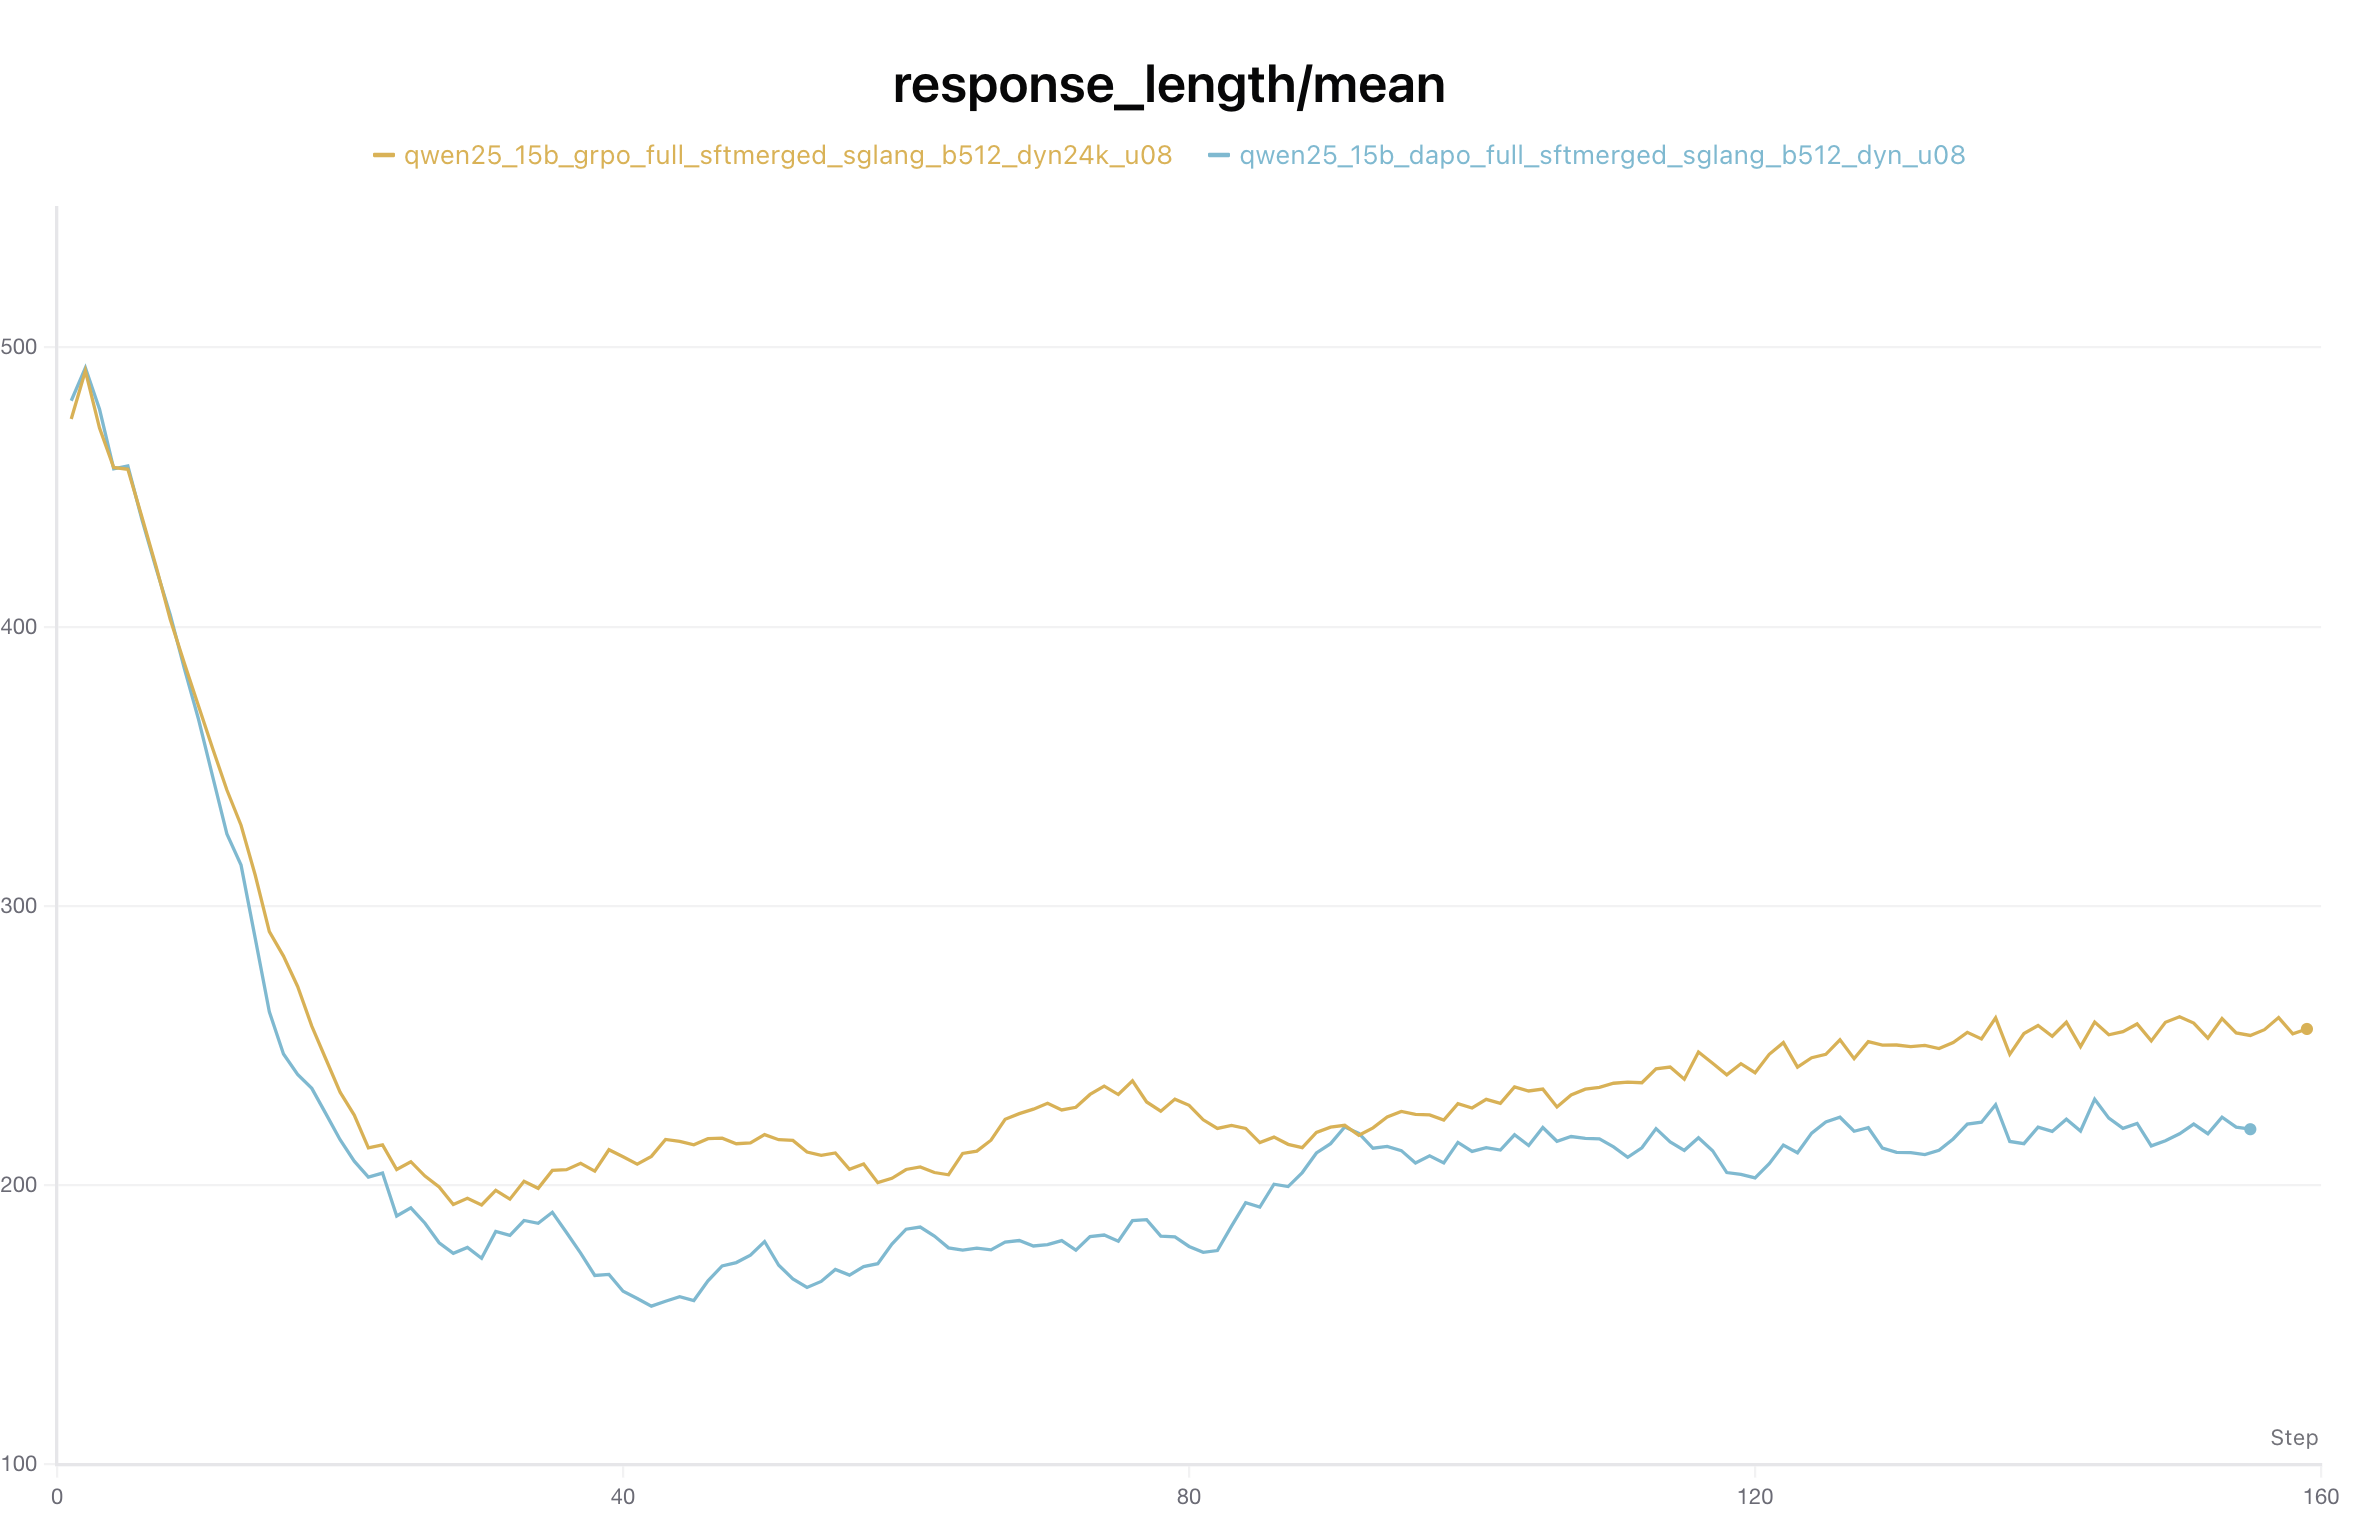
\includegraphics[width=0.85\linewidth]{figures/response_len.png}
\caption{Mean response length during S3 training for GRPO (orange) vs.\
DAPO (blue). Both curves first contract from a long-output prior to a
tighter regime in the first $\sim$20 steps, then re-expand modestly. GRPO
settles around 250+ tokens, DAPO around 220+, indicating that GRPO
preserves slightly longer reasoning traces under the same length budget.}
\label{fig:resplen}
\end{figure}

\begin{figure}[h]
\centering
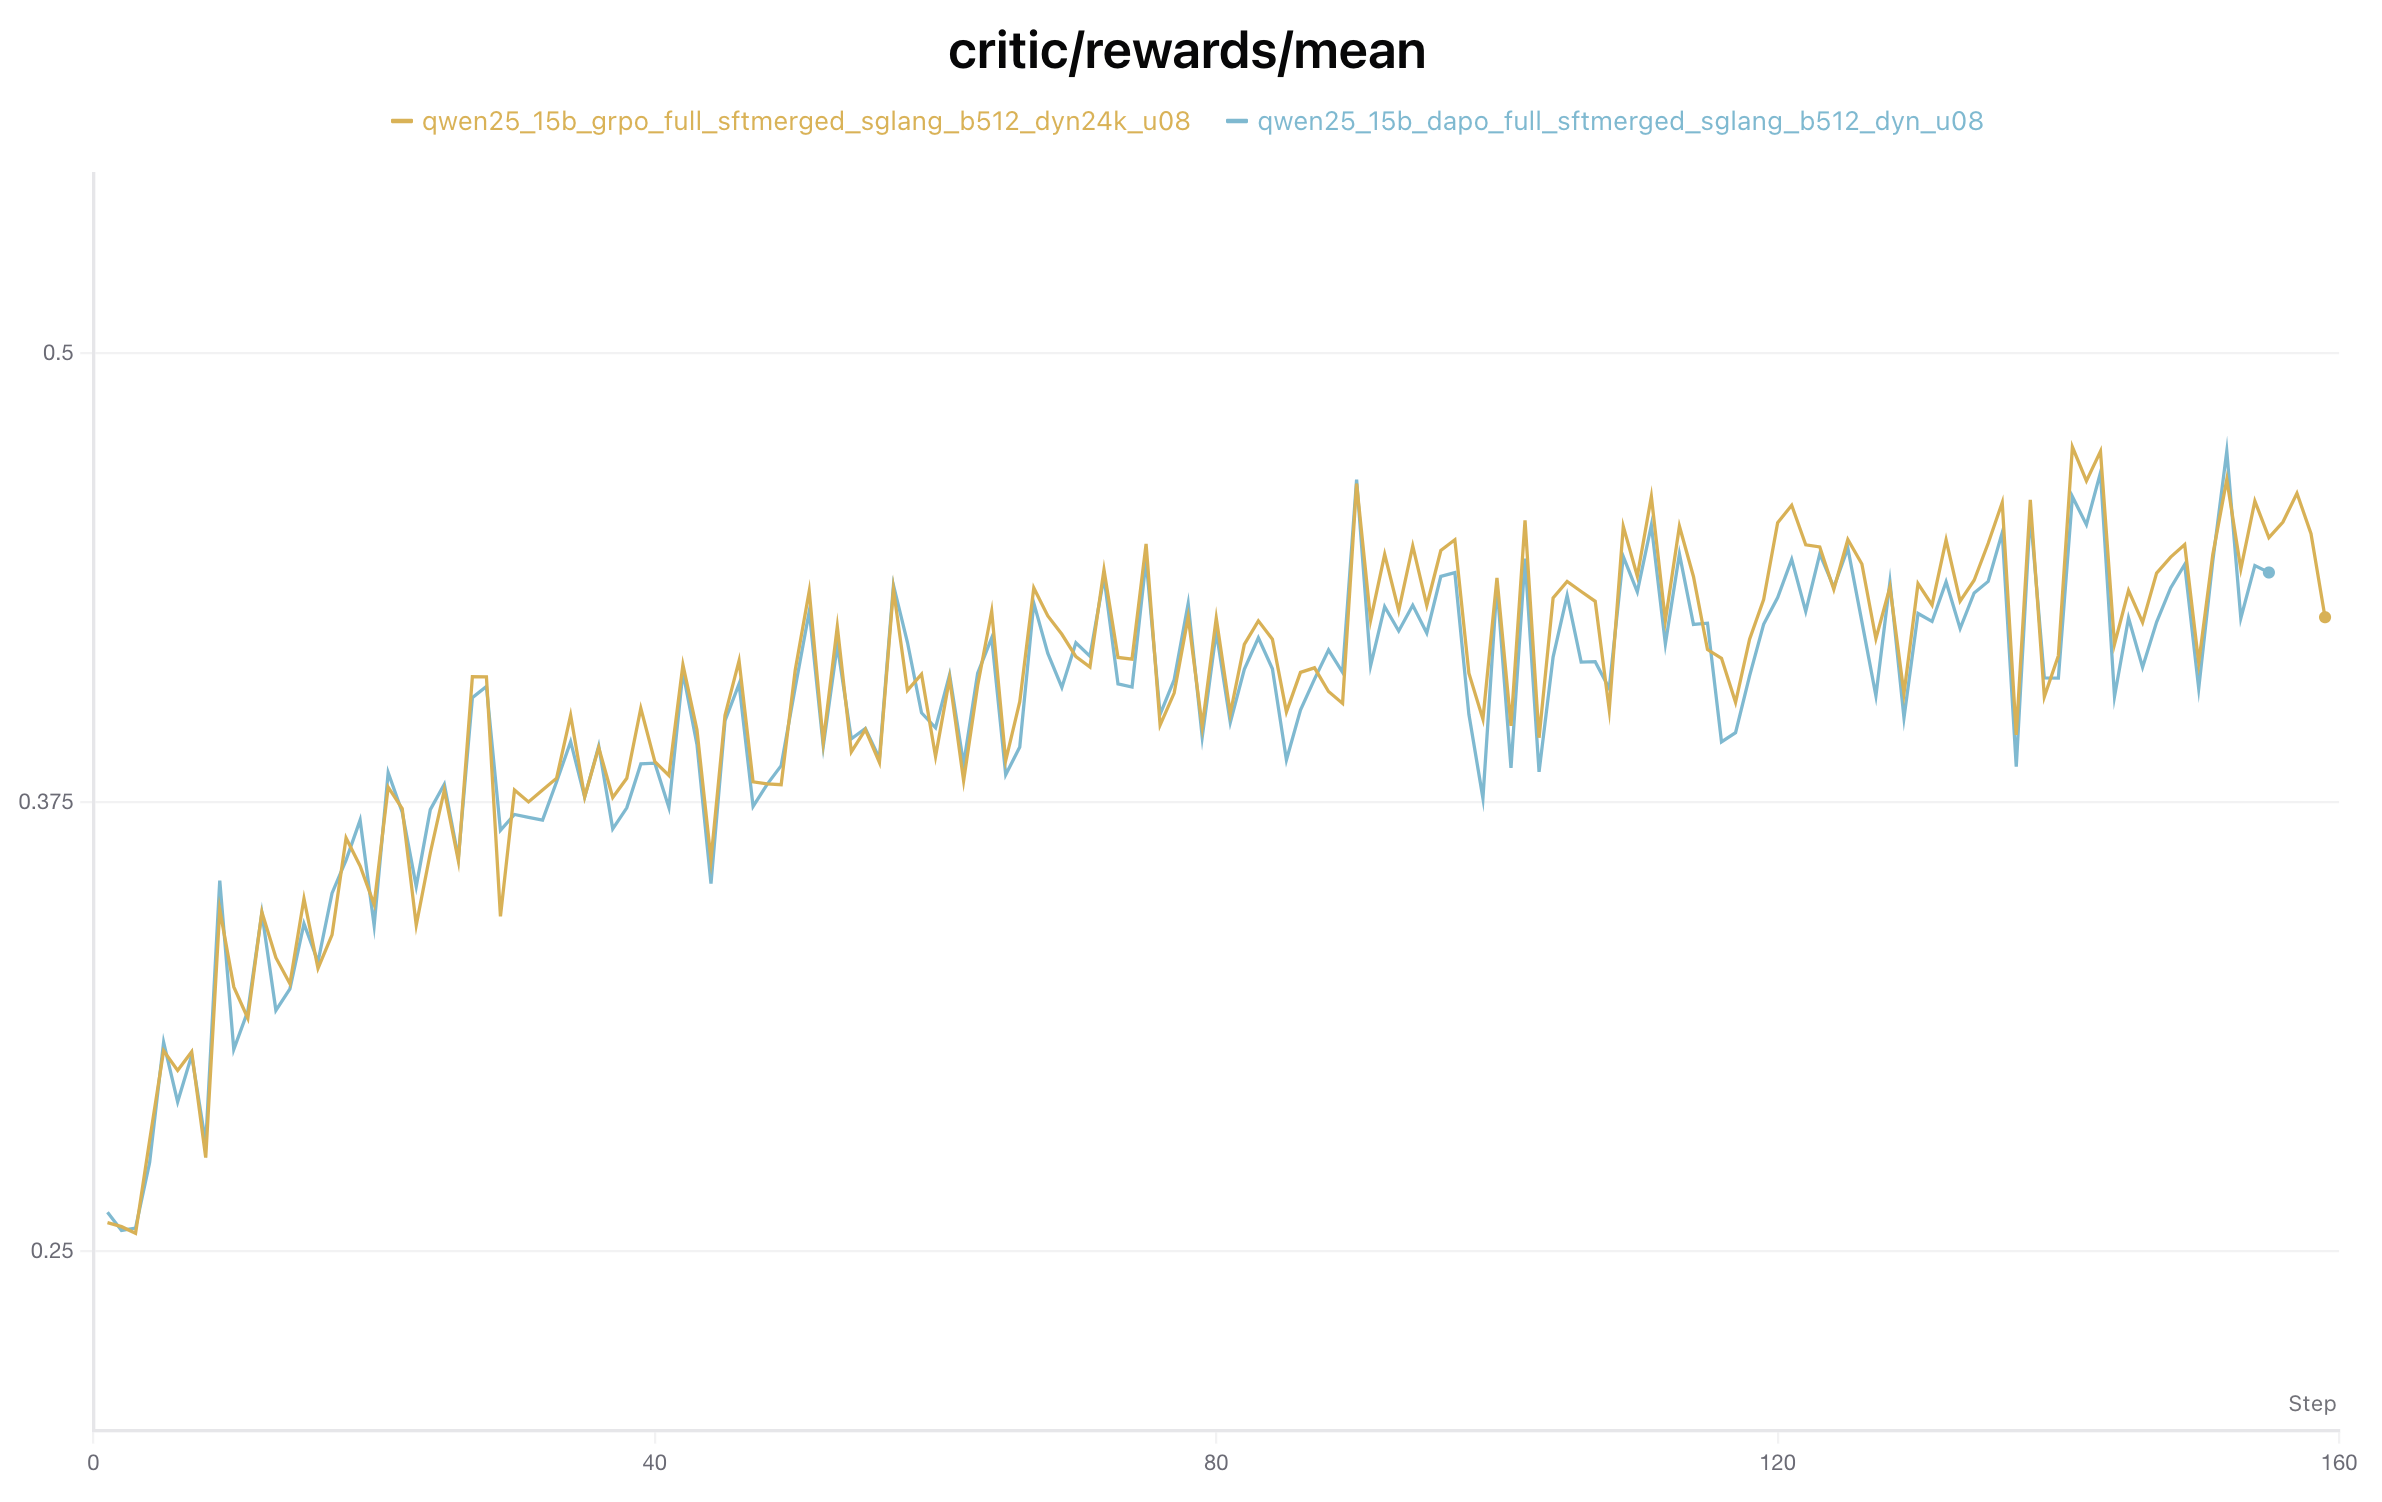
\includegraphics[width=0.85\linewidth]{figures/reward.png}
\caption{Mean reward $\mu_R$ during S3 training. Both algorithms climb
from $\approx 0.25$ to the $0.42$--$0.46$ band and stay there. The two
trajectories are very similar, with GRPO ending marginally higher.}
\label{fig:reward}
\end{figure}

\Cref{fig:resplen,fig:reward} together suggest that GRPO and DAPO behave
qualitatively similarly under our reward shape and hyperparameter range:
both contract their output, then learn to produce an answer-line ending
that consistently triggers $\rExact$ or $\rEquiv$, and both plateau in the
same reward band. The choice between them is therefore more about
engineering preferences than absolute performance, which is reflected in
the close numbers reported in \cref{sec:results}.
